\chapter{SEMANTICS-AIDED LONG-TERM LOCALIZATION}

\section{Introduction}
 
In recent years, the limitations of pure geometric maps built from conventional \acrshort{vslam}/\acrshort{vo} has been recognized and the idea of semantic mapping has gained more and more popularity. 
With the recent development of deep learninig techniques, state-of-the-art semantic segmentation networks have shown impressive repeatability under perception changes, e.g. multiple weathers, day and night, and across seasons. 
Such appearance change invariance makes the semantics become relevant for motion estimation, especially benefitial for the long-term localization applications. 

Long-term visual localization is the problem of estimating the camera pose of a query image relative to 3D scene structure across appearance variations due to changes in time, weather, or seasons \cite{sattler2018benchmarking}. 
It is an important enabling module for robotic application domains involving long-term deployments in outdoor environments and others with highly variable visual conditions  \cite{dayoub2008adaptive,krajnik2014long,valgren2010sift,stenborg2018long}.

Classical approaches to localization rely on the local, image feature descriptors to establish 2D-3D correspondences for pose estimation \cite{liu2017efficient,geppert2019efficient,sarlin2019coarse}.
Continued use of these approaches requires robust local descriptors sensitive to structural differences but not to changes in visual conditions.
However, traditional feature descriptors are typically optimized for use when the query and database images are taken under similar visual conditions, as the emphasis is on robustness to the viewpoint \cite{balntas2017hpatches,schonberger2017comparative}.
Mismatch errors increase if the localization and mapping stages occur under different visual circumstances.
In contrast, data-driven approaches to feature detection and description are capable of establishing methods robust to both disturbance sources 
\cite{detone2018superpoint,dusmanu2019d2,revaud2019r2d2,luo2020aslfeat}. 
Metric learning techniques have contributed to these outcomes \cite{mishchuk2017working}, since a deep neural network training process generates keypoint representations adapted to the data.  
Unfortunately, generalizing beyond the data remains problematic.

\begin{figure}[t] 
 	\centering
  	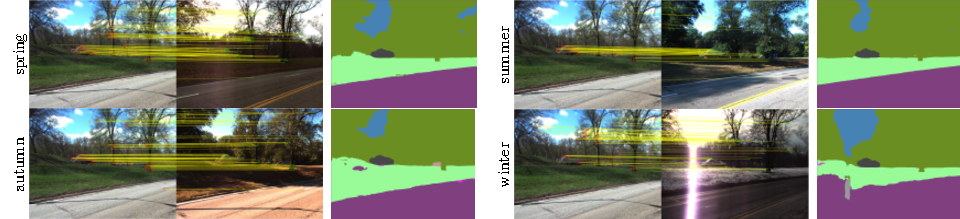
\includegraphics[width=0.8\linewidth]{figures/learning/intro.pdf}
    \caption[Matches and Semantics from {\em DLSSNet}]{\textbf{Matches and Semantics from {\em DLSSNet}.} {\em DLSSNet} extracts keypoints with multi-level descriptors for image matching across significant appearance variations due to seasonal changes. Semantic segmentation is a side output.
    \label{fig:learning_intro}}
\end{figure}

Another means to relax the sensitivity while preserving discriminatory power for point plus feature descriptor solutions has been to implement semantics-aided localization strategies.  
The introduction of high-level semantic information supplements the low-level descriptor information, resulting in fewer mismatches and more robust visual localization. 
This multi-level integration is beneficial, however, there are some non-negligible design parameters need to be taken care of:
\begin{enumerate}
	\item The integraiton of multi-level information from deep network increases the complexity of the network, which creates more annotation demands and requires attention with regards to how the layers should be trained due to the coupling.
Consequently, the influence of network structure and learning methods on performance has not been fully explored.  
	\item The efficacy of high-level guidance on top of multi-level description learning is unclear, meaning that evidence-supported guidance concerning network design for localization is nonexistent.  
	\item Task-specific fine-tuning of semantics or semantics-augmented description learning has trouble addressing annotation needs or indicating how to reduce human-annotation demands. 
\end{enumerate}


In this chapter, we concentrate on two key developments towards the above-mentioned problems:
\begin{enumerate}
	\item We fill this gap by evaluating multi-level descriptors w or w/o high-level guidance in the context of long-term localization.  
Based on the results, we choose the best-performed network presented in this section.  
In particular, we show that the semantic segmentation and local feature description can be simultaneously learnt within the hierarchy of a single deep network pipeline.
A descriptor segmentation module jointly learns semantic descriptors and
cluster means using a standard segmentation loss.
The augmented multi-level descriptors, trained in an end-to-end manner, provide a more stable high-level representation for local feature dis-ambiguation as compared to other architectures.
	\item We provide a pre-training process approach using standard semantic segmentation datasets, after which the network may be fine-tuned using only 2D-2D matches. 
The two-part process permits the domain-specific adaptation of the learnt localization module for addressing the challenges of long-term localization, so that training complexity and data annotation needs are not limiting factors. 
Modifications have been made to facilitate efficient task-specific fine-tuning without extra semantic annotations.  
\end{enumerate}

\section{Background}

\noindent \textbf{Deep Feature Learning}
Given that the classical paradigm for visual localization involved sequential feature detection followed by feature description, deep learning {\em detect-then-describe} pipelines naturally arose.  
Reflecting a similar sequential nature, detector networks first generate score maps for keypoint selection \cite{verdie2015tilde, savinov2017quad, barroso2019key}. 
Next, small image patches centered at keypoint locations are cropped and input to descriptor networks to generate keypoint descriptions \cite{mishchuk2017working, tian2017l2, he2018local, keller2018learning, luo2018geodesc, mishkin2018repeatability, mukundan2019explicit, ebel2019beyond, tian2019sosnet}.  
The networks are independent of each other and trained that way.  
Unified architectures describe sequentially applied networks that can be jointly trained in an end-to-end manner \cite{yi2016lift, ono2018lf}. 
Though simplifying the training process, these unified architectures preserve network complexity. 
Importantly, they continue to process descriptors at the image patch level, which prevents learning contextual cues outside of the local patches.


For modern deep networks with high parametric degrees of freedom, it is sensible that both detection and description could be encoded within the same network and jointly learnt. 
This joint design describes a \textit{detect-and-describe} deep feature learning approach that operates on full-sized images as opposed to patches \cite{detone2018superpoint,revaud2019r2d2,dusmanu2019d2,luo2020aslfeat}.
Using a single encoding element improves computational efficiency due to shared weights. What distinguishes the methods are the self-supervised learning tactics and detector design.
SuperPoint \cite{detone2018superpoint} uses a dual branch decoder with a heatmap keypoint detector on one of the decoder branches. 
R2D2 \cite{revaud2019r2d2} has branches for repeatability and reliability maps that together recover keypoints of interest. 
The idea is to identify points that will almost always be detected and whose descriptions will be discriminative.  
Theoretically, image-wide convolutional structures permit learning of high-level contextual information, however contextual learning is limited by the stencil sizes.  
The learnt features are observed to still have fairly localized representations of image structure. 

D2-Net \cite{dusmanu2019d2} avoids a separate detection branch and builds a sequential process to perform keypoint detection directly from the pixel descriptors.
It is more accurately called a {\em describe-to-detect} process since the descriptor outputs influence the detector. 
Detections based on feature vector outputs should induce higher-level feature learning that is less localized in nature. 
If so, it comes at the price of reduced keypoint localization accuracy. 
ASLFeat \cite{luo2020aslfeat} instead modifies the {\em
detect-and-describe} process by outputting multiple keypoint detector heatmaps at different layers within the network to recover low-, mid-, and high-level structure. 
Their fusion acts like a multi-scale keypoint detection process. 
Additional elements in the network provide robustness to
image deformation arising from viewpoint changes.
What is ultimately captured at the "high" level will still be constrained by the stencils across the layers.

 
\noindent \textbf{Semantics-Aided Localization}
One form of higher-level contextual information is semantic scene knowledge.  
Semantic labels act as a weak supervisory signal to distinguish between correct and incorrect correspondences.  
A common strategy is to incorporate semantic labels into the matching stage of localization, where each 2D-3D match is assigned to a semantic consistency score \cite{toft2018semantic,shi2019visual} to influence the \acrshort{ransac} sampling for robust pose estimation. 
The bottleneck of such methods is the number of available classes, as the quantity directly translates to the discriminative power of potential matches. 
Self-supervised semantic learning methods that generate fine-grained segmentation networks overcome this problem \cite{larsson2019fine}.

Joint, multi-level descriptors combine the complementary information from semantics and geometric local features during the feature learning process.  
One group of them \cite{luo2019contextdesc, hong2020learning} directly combines the features from off-the-shell networks trained on low- or high-level tasks for multi-level keypoint description.
Although the unified frameworks have been delicately designed for end-to-end training, the fine-tuning of high-level representation still faces an efficacy problem due to multi-network multi-task learning
needs \cite{luo2019contextdesc}.
Alternatively, multi-level descriptors concatenated from different stages of the network improve object detection, semantic segmentation, and part labeling \cite{hariharan2015hypercolumns}.
Following this work, a hierarchical metric learning pipeline is proposed \cite{fathy2018hierarchical}, and improved \cite{spencer2019scale}, to make the multi-level descriptors trainable end-to-end using simple correspondence contrastive loss.
Other methods try to learn the multi-level descriptors in conjunction with auxiliary high-level tasks: the pixel-wise descriptors are extracted and concatenated from multiple layers of image retrieval network for localization tasks using merely image-level supervision \cite{germain2019sparse}. 
Later, point-wise supervision \cite{sarlin2019coarse} is incorporated along with the image correspondences for fine-grained point description learning, but using single-level descriptions. 


\section{Datasets}

{\em DLSSNet} is trained from image pairs gathered from three different sources.
A semantic segmentation dataset (Cityscapes \cite{cordts2016cityscapes}) with synthetically generated pairs initialize the descriptors and clusters.
Later, a visual odometry dataset (KITTI \cite{geiger2012we}) uses sequential images as pairs to refine the network, especially for local feature learning. 
Finally, the cross-season localization datasets (RobotCar-Seasons \cite{Maddern2017IJRR} and Extended CMU-Seasons \cite{Badino2011}) with ground-truth cross-seasonal point correspondence
(Cross-Seasons Correspondence Dataset \cite{larsson2019cross}) fine-tune the whole network for cross-season localization. 
\ref{tbl:learning_datasets} summarizes the dataset information for training and testing.
The Extended CMU-Seasons datasets splitting is based on the availability of corrrespondences for training, where the slices with ground-truth correspondence serves as training data and the rest as testing data.

\begin{table}
	\centering
	\caption[Dataset Information]{ Dataset Information 
	\label{tbl:learning_datasets}}
	\begin{tabular}{cccccc}
\hline
Dataset                                                                           & Condition & \begin{tabular}[c]{@{}c@{}}Training\\ Seq\end{tabular} & \begin{tabular}[c]{@{}c@{}}Testing \\ Seq\end{tabular} & \begin{tabular}[c]{@{}c@{}}\#Training\\ Pairs\end{tabular} & \begin{tabular}[c]{@{}c@{}}\#Testing\\ Pairs\end{tabular} \\ \hline
Cityscapes  \cite{cordts2016cityscapes}                                                                      & urban     & all                                                    & -                                                      & 5,000                                                      & -                                                         \\
KITTI \cite{geiger2012we}                                                                            & urban     & 05-08                                                  & -                                                      & 10,000                                                     & -                                                         \\
RobotCar \cite{Maddern2017IJRR}                        		                                                                            & urban     & all                                                    & -                                                      & 6,511                                                      & -                                                         \\
\multirow{3}{*} {CMU \cite{Badino2011} }                                                                                       & urban     & 6-8                                                    & 2-5                                                    & \multirow{3}{*}{28,766}                                    & \multirow{3}{*}{46,569}                                   \\
                                                                                  & suburban  & 9-13                                                   & 14-17                                                  &                                                            &                                                           \\
                                                                                  & park      & 21-25                                                  & 18-20                                                  &                                                            &                                                           \\ \hline
	\end{tabular}
\end{table} 


\section{Learning Multi-Level Description and Semantic Segmentation}

\begin{sidewaysfigure}[htbp] 
  	\centering
  	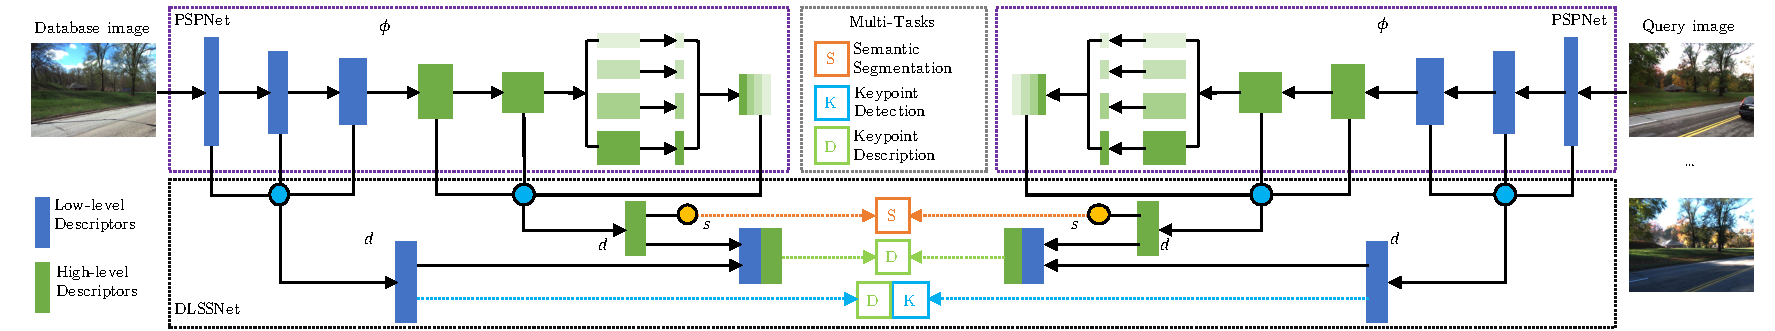
\includegraphics[width=\linewidth]{figures/learning/architecture.pdf}
    \caption[Architecture and Training Strategy of {\em DLSSNet}]{ \textbf{Architecture of {\em DLSSNet}.} \textbf{Top}: Our proposed network consumes a single image as input, which simultaneously predicts low-level keypoint detection and description, high-level semantic segmentation, and multi-level description within a single network. \textbf{Bottom-Left}: Multi-level feature fusion and descriptor segmentation modules. \textbf{Bottom-Right}: Training Pipeline of {\em DLSSNet} can be expressed as a two-stage procedure, where a supervised pre-training and a weakly-supervised task-specific fine-tuning are interleaved for semantics-stabilized description learning in the context of long-term localization.
    \label{fig:learning_arch}}
\end{sidewaysfigure}


% Overall structure
As illustrated in \ref{fig:learning_arch}, our proposed Descriptor Learning and Semantic Segmentation Network ({\em {\em DLSSNet}}) is built upon PSPNet \cite{li2018pyramid} pretained on semantic segmentation tasks. 
The feature embeddings from different stages of the network are first fused into two integrated descriptors. 
Then, the resultant low- and high-level descriptors are utilized to accomplish three complementary tasks: 
low-level {\em detection-and-description}, high-level semantic segmentation, and 
multi-level description.

Our network design takes advantage of the inherent hierarchy of \acrshort{cnn} to learn semantic and local geometric features from different layers of a single deep network \cite{hariharan2015hypercolumns}.  
Local geometric features identify low-level structures, such as corners, edges, etc., for keypoint localization and description.
Contextual features, learned from semantic segmentation tasks, encode the high-level regional information into point description.  
The multi-level concatenated descriptors formulate a richer visual representation for keypoint matching.

\subsection{Multi-Level Feature Fusion}
% Overall procedure
The main task of our proposed feature fusion module is to establish a low-level geometric local descriptor and a high-level semantic descriptor by fusing feature embeddings from multiple network layers.
We first divide deep features extracted from the bottlenecks (5 layers) and pyramid pooling module (1 layer) of PSPNet in a tuple format as shown in \ref{fig:learning_arch}. 
Then, the two groups of feature embeddings are fed into our proposed feature fusion module for descriptor formulation. 
We group feature in a tuple format based on the observations that (1) state-of-the-art feature learning networks either truncate deep models after the third blocks \cite{dusmanu2019d2} or utilize very shallow networks \cite{detone2018superpoint,revaud2019r2d2,luo2020aslfeat} for low-level high-resolution local description learning, and (2) simple fusion of lower-level features into high-level ones tend to be less effective for
semantic segmentation \cite{zhang2018exfuse}.


% Detailed structure
As illustrated in \ref{fig:learning_arch} (bottom-left), our proposed multi-level feature fusion module takes the multi-level feature embeddings $\{ \phi_{l-1}, \phi_{l}, \phi_{l+1} \}$ with different resolutions and channels as inputs and outputs a fused descriptor $\mathbf{d}$ for subsequent tasks. 
Channel reduction and size adaption modules first resize the feature maps to equal channels and same spatial resolution through individual {\em conv1x1+bn+relu}
computations and {\em bilinear interpolation}, respectively. 
For computational efficiency, we implement feature summation, instead of concatenation, to fuse the generated features into a tensor of 128 channels at each resolution.  
The integrated descriptors are finally mapped into Spherical space for dense description formulation through channel-wise {\em L2-normalization}.
The fused descriptors capture either geometrical information from bottom network layers or semantic cues from top ones. 
%for later tasks.

\subsection{Learning Low-Level Detection-and-Description}
The low-level {\em description-and-detection} module here builds on D2-Net \cite{dusmanu2019d2} to jointly learn a descriptor and keypoint detector using ground-truth point matches from \acrshort{sfm} models.
Considering the low-level natures of keypoint detection, 
{\em detection-and-description} uses low-level descriptors that not only maintain spatial resolution but also learn local details for accurate keypoint localization.


\subsubsection{Detection}
Given the low-level dense descriptor $\mathbf{d} \in \mathbb{R}^{H \times W \times C}$, the local spatial and channel-wise score maps, $\alpha$ and $\beta \in \mathbb{R}^{H \times W \times C} $, are computed for soft keypoint detection:
\begin{equation} \label{eq:learning_d2localscore}
\alpha_{ij}^k = \frac{exp(d_{ij}^k)}{\sum_{(i',j')\in \mathcal{N}(i,j)}
exp(d_{i'j'}^k)}, \ \ 
\beta_{ij}^k = \frac{exp(d_{ij}^k)}{\max_{k'} exp(d_{ij}^{k'})}
\end{equation}
where $\mathcal{N}(i,j)$ is a set of 9 neighboring pixels around coordinate $(i,j)$. 
Finally, the saliency score map $\mathbf{s} \in \mathbb{R}^{H \times W}$ weights the pixel-wise description loss after image-wise \textit{L1-normalization}:
\begin{equation} \label{eq:learning_d2detectionscore}
s_{ij} = {\gamma_{ij}} \,\big/ {\sum_{(i',j')} \gamma_{i'j'}}, \ \textrm{where} \ \gamma_{ij} = \max_k \alpha_{ij}^k \beta_{ij}^k
\end{equation}

\subsubsection{Learning Detection-and-Description}
Given a set of correspondences $\mathcal{C}$ from an image pair ($I, I'$), the {\em detection-and-description} loss of D2-Net \cite{dusmanu2019d2}, maximizes description distinctiveness at
most repeatable keypoint locations:
\begin{equation} \label{eq:learning_d2loss}
\mathcal{L}_{dl}(I,I') = \frac{1}{|\mathcal{C}|} \sum_{c \in \mathcal{C}}\frac{s_c s_c'}{\sum_{k \in \mathcal{C}} s_k s_k'} \mathcal{M}(\mathbf{d}, \mathbf{d}')
\end{equation}
where $s$ and $s'$ are detection score maps \eqref{eq:learning_d2detectionscore} calculated from image $I$ and $I'$, respectively. 
$\mathcal{M}(\cdot, \cdot)$ is the ranking loss for description learning given a pair of descriptors $\mathbf{d}$ and $\mathbf{d}'$ of point correspondence. 

Following the suggestion from ASLFeat \cite{luo2020aslfeat}, we utilize the hardest-contrastive loss \cite{choy2019fully} instead of hardest triplet loss in D2-Net \cite{dusmanu2019d2} for better convergence: 
\begin{equation} \label{eq:learning_d2distance}
\mathcal{M}(\mathbf{d}, \mathbf{d}')
  = \mathcal{M}(\mathbf{d}, \mathbf{d}')_+ 
    + \mathcal{M}(\mathbf{d}, \mathbf{d}')_-
\end{equation}
where
\begin{equation} \nonumber
\begin{split}
  \mathcal{M}(\mathbf{d}, \mathbf{d}')_+ 
    & = \max(0, D(\mathbf{d}, \mathbf{d}')-m_p) \\
  \mathcal{M}(\mathbf{d}, \mathbf{d}')_- 
    & = \max(0, m_n - \min(
      \min_{\bar{\mathbf{d}} \neq \mathbf{d}}D(\bar{\mathbf{d}}, \mathbf{d}'),
      \min_{\bar{\mathbf{d}}' \neq \mathbf{d}'}D(\mathbf{d},\bar{\mathbf{d}}')
      ))
\end{split}
\end{equation}
for $D(\cdot,\cdot)$ the distance between two descriptors. $m_p$ and $m_n$ are the positive and negative margins.

\subsection{Learning High-Level Description Segmentation}
Semantic segmentation, as an auxiliary task, is trained at deeper layers of the network to learn the high-level representation. 
The emphasis is on formulating and stabilizing the semantic descriptors for domain-specific applications. 
As such, no special effort is made to improve semantic segmentation performance. 
The uniqueness of our training is that the descriptor segmentation module jointly learns semantic descriptors $\mathbf{d}$ and cluster means $\mu$ in an end-to-end manner, where the probability distribution of semantic assignments is computed directly from learnt descriptors. 
It can be easily trained using point correspondence loss and supervised or weakly-supervised semantic segmentation loss.


\subsubsection{Descriptor segmentation}
Inspired by the recent advance of \acrlong{dec} (\acrshort{dec}) \cite{xie2016unsupervised}, a descriptor segmentation module is proposed to jointly learn the high-level descriptors $\mathbf{d} \in {H \times W \times C}$ and cluster centers $\mu \in {C \times K}$. 
It is achieved by mapping the descriptors from the spherical space to a lower-dimensional feature space that iteratively optimizes the semantic assignments $s\in {H \times W \times K}$.

Specifically, we use the t-distribution as a kernel to measure the similarity $s$ between descriptor $\mathbf{d}$ and $k^{th}$ cluster centroid $\mu_k$ at $(i,j)$ coordinate:
\begin{equation} \label{eq:learning_tdistribution}
s_{ij,k} = \frac{(1+\| \mathbf{d}_{ij,k}-\mu_k \|^2)^{-1}}{\sum_{k'} (1+\| \mathbf{d}_{ij,k'}-\mu_{k'} \|^2)^{-1}} =
\frac{(3 - 2\mathbf{d}_{ij,k}^T\mu_k)^{-1}}{\sum_{k'} (3 - 2\mathbf{d}_{ij,k'}^T\mu_{k'})^{-1}}
\end{equation}
As such, the semantic assignment $s$ can be efficiently computed using standard convolutional operations \textit{conv1x1+softmax} as shown in \ref{fig:learning_arch} (bottom-left), where the column weights of \textit{conv1x1}, after \textit{L2-normalization}, serve as cluster centers $\mu$ for joint optimization.

\subsubsection{Learning Semantic Segmentation}
Though \acrshort{dec} is designed for unsupervised learning, we advocate for supervised segmentation since it improves descriptor learning, as long as the ground-truth labels are available, due to the stability
induced by supervision. 
To enable task-specific fine-tuning without additional data annotations, a weakly-supervised semantic segmentation pipeline is introduced to achieve efficient domain adaption.  
The losses for supervised and weakly-supervised training are detailed here.

The standard cross-entropy loss is chosen to supervise the model training using ground-truth semantic labels:
\begin{equation} \label{eq:learning_crossEntropy}
\mathcal{L}_{ce}(I) = \frac{1}{|I|} \sum_{(i,j) \in I} l_{ij}^T \log (s_{ij})
\end{equation}
where $s$ stands for probability distribution of semantic assignments $s$ computed from our proposed descriptor segmentation, and $l$ is the
ground-truth semantic labels. 

For the cases that the semantic annotation is unavailable, the 2D-2D correspondences from \acrshort{sfm} reconstructions can be used to enforce labeling consistency between acquired images as long as one of the images is taken at a similar condition as pre-trained datasets. 
As such, the ground-truth labels can be substituted by one-hot pseudo-label $\hat{l}$ calculated from the confidence of semantic assignment $s$ as:
\begin{equation} \label{eq:learning_pCrossEntropy}
\mathcal{L}_{pce}(I,I') = \frac{1}{|\mathcal{C}|} \sum_{c \in \mathcal{C}} \hat{l}_c^T \log (s_c)
\end{equation}
The pseudo-labels should be calculated from database images in localization datasets captured in favorable conditions \cite{larsson2019cross}. 


\subsubsection{Learning Point Correspondence}
The priority of the descriptor segmentation module is to learn point-wise semantic descriptors for robust matching, where the semantic segmentation loss only enforces region-to-region similarity. To encourage a fine-grained high-level description, the point correspondence loss are incorporated for fine-grained semantic representation learning:
\begin{equation} \label{eq:learning_pc}
\mathcal{L}_{pc}(I,I') = \frac{1}{|\mathcal{C}|} \sum_{c \in
\mathcal{C}} \mathcal{M}(d_c,d_c')_+ \,.
\end{equation}

\subsection{Learning Multi-Level Description}
There are several options for merging the low-level geometric and high-level semantic descriptors. 
One is to combine two descriptors through element-wise \textit{summation} and \textit{L2-normalization} like in the feature
fusion module and in \cite{luo2019contextdesc}.
In the presence of the semantic gap between two types of features, it is questionable that summation is capable of preserving the complementary information due to loss of separability.
Feature concatenation is a better option at the expense of increased computational cost at the matching stage
\cite{hariharan2015hypercolumns, fathy2018hierarchical,
spencer2019scale, germain2019sparse, min2019hyperpixel}. 
Having the keypoint detection scores \eqref{eq:learning_d2detectionscore} and the concanated descriptors, we train our multi-level descriptors in an
end-to-end manner using the {\em detection-and-description}, hardest-contrastive loss in \eqref{eq:learning_d2loss}.

\section{Training and Fine-Tuning}

\ref{fig:learning_arch} (bottom-right) depicts the training process, with semantic segmentation pre-training, followed by task-specific fine-tuning with weak supervision from 2D-2D correspondences. 
The two tasks iteratively optimize the description.
To facillitate both training and fine-tuning, the combined loss is implemented:
\begin{equation} \label{eq:learning_trainingloss}
\mathcal{L} = \lambda^{l}\mathcal{L}^{l}_{dl} + \lambda^{h}(\mathcal{L}^{h}_{(p)ce} + \mathcal{L}^{h}_{pc}) + \mathcal{L}^{m}_{dl}
\end{equation}
where the superscripts $l$, $h$, and $m$ refer to low-, high-, and multi-level tasks, and $\lambda^{(\cdot)}$ are weighting terms. 

{\em DLSSNet} is pre-trained using semantic segmentation datasets in conjunction with a self-supervised synthetic image pairs. 
The ground-truth point correspondences are computed along with the randomly transformed image and semantic labels.
Pre-training helps to initialize all three components of {\em DLSSNet}. 
A two-step pre-training procedure for descriptor learning initializes cluster centers without significantly altering the high-level representations. 
First, we fix the weights of PSPNet and optimize the introduced modules to convergence. 
Second, the whole network is jointly optimized.

Using domain adaptation ideas \cite{larsson2019cross}, we implement a weakly-supervised training pipeline to alleviate the demand for manually created annotations for long-term localization.  
The 2D-2D point correspondence from \acrshort{sfm} enforces semantic and geometric consistency for domain-specific point descriptor fine-tuning.
The pipeline takes advantage of the observation that the database images in long-term localization datasets are usually captured during
favorable conditions.
It inherently enables knowledge transfer from easy to hard.  
To this end, the cross-entropy loss is optimized with pseudo-labels inferred from semantic assignments of database images.  
Implementing an interleaved training procedure maintains a stable semantic representation.  
It prevents trivial solutions during optimization of the high-level representations\cite{larsson2019cross}.  

\section{Evaluation}
In this section, we investigate the effects of key parameters on the design of {\em DLSSNet}.
Finally, we benchmark {\em DLSSNet} on the task of cross-season localization. 


\subsection{Implementation Details}
This section gives implementation details about training that most affect performance, and about evaluation.

\subsubsection{Training Details}
% backbone
As a starting point, the PSPNet \cite{li2018pyramid} (ResNet-101), pre-trained on Cityscapes \cite{cordts2016cityscapes} dataset, are selected for cross-season point description learning.
% GT correspondence
To obtain dense ground-truth correspondence, image sequences are first fed into an \acrshort{sfm} pipeline for dense reconstruction. 
Ground-truth correspondences are computed by estimating either 2D-3D or 3D-3D matches between image pairs.  
The 2D-3D matching strategy is usually applied to scenes with minor appearance changes, where standard 2D features will work.  
The 3D-3D method is used for long-term localization datasets, since 2D features are unreliable under large appearance changes.
% GT semantic segmentation
The ground-truth semantic annotations are either provided by semantic segmentation datasets or directly inferred from the network outputs as pseudo-labels in a weakly supervised pipeline. 

% preprocessing
As a preprocessing step, image pairs are first standardized to zero-mean unit-norm tensors, then augmented using random photometric transformations, such as brightness, contrast, and color noise.
% optimization
During the optimization, the loss described in \eqref{eq:learning_trainingloss} is computed from pairs with at least 50 point matches, and with loss balance factors $\lambda^l = \lambda^h = 0.4$. 
The SGD optimizer is used with a learning rate of $0.1$.
% details about training pipeline 
{\em DLSSNet} is trained on semantic segmentation tasks, CityScapes, with synthetic pairs for 30 epochs, where the synthetic data is simple and fast for rendering. 
Later, it is fine-tuned on KITTI, RobotCar-Seasons, and Extended CMU-Seasons for 50 epochs each for cross-season specific description learning.  


\subsubsection{Localization pipeline}
Evaluation of cross-season localization uses a two-step pipeline. 
First, dense SfM models are generated from COLMAP \cite{schoenberger2016sfm} using the \acrlong{mvs} (\acrshort{mvs}) \cite{schoenberger2016mvs} pipeline as a default setting. 
Then, the query images are registered to 3D maps (image + depth map) using customized features.
The 2D-3D matches, defined as mutual nearest neighbors, are used to realize camera poses using n-point-pose solver \cite{kneip2011novel}
inside a \acrshort{ransac} loop \cite{fischler1981random}.   
To compare different deep features we use: 
%\issue{For a fair comparison between different deep features we use:}
(1) provided ground-truth poses to generate image pairs; and 
(2) SIFT \cite{lowe2004distinctive} features to reconstruct dense depth maps using COLMAP with \acrshort{mvs} option for all reference images.

\subsubsection{Evaluation protocal}
Camera localization is evaluated using camera pose recall, that is, the percentages of successfully localized images using the coarse-to-fine error tolerances $(0.5m, 2deg) / (1m, 5deg) / (5m, 10deg)$ for the ablation study and performance evaluation.

\subsection{Ablation Study}
To understand network design properties, we study the impact of:
(1) different training datasets; 
(2) multi-level description fusion; 
(3) semantic description; and 
(4) high-level guidance from semantic segmentation using Extended CMU-Seasons dataset.
\ref{tbl:learning_ablation} lists the ablation study outcomes.

Unlike state-of-the-art networks for large-scale web image retrieval, {\em DLSSNet} is trained using autonomous driving datasets for applicability of
the semantic annotations.  
The table first lists percentages for successfully localized images when training on subsets of the training corpus.
Synthetically generated image pairs don't provide satisfying performance (row 1). 
Incorporating real image pairs from KITTI sequences enables significant improvements at all scenes, while the fine-tuning at RobotCar-Seasons
and Extended CMU-Seasons give another boost especially for park scenes
(rows 2 \& 3).

A major claim of this work is that multi-level descriptors combine the complementary strength of low- and high-level features for better long-term localization. 
The second part of the ablative study analyzes this proposal by comparing the single- and multi-level descriptors.  
The evaluation reveals that shallower features provide more accurate camera pose estimation than deeper ones (rows 4 \& 5), while the high-level component, although less discriminative, provides sufficient complementary information to boost performance (row 6).
  
A third claim is that semantic segmentation, as high-level guidance, helps to learn better descriptors for camera relocalization. 
We compare the features learned w \& w/o the auxiliary semantic segmentation task (rows 7 \& 8). 
High-level descriptors learned from human-defined semantic segmentation tasks do provide better performance.
Compared to semantic confidence of pre-defined labels, semantic descriptors learns a richer description for robust matching (rows 9 \& 10). 
Similar to the finely-grained segmentation \cite{larsson2019fine}, the learned semantic descriptor enforces a finer data association during keypoint matching.
 
\begin{table}[t]
	\centering
	\caption[Ablative Study of {\em DLSSNet}]{ Ablative Study of {\em DLSSNet} 
	\label{tbl:learning_ablation}}
	\begin{tabular}{cccc}
\hline
\multirow{2}{*}{\begin{tabular}[c]{@{}c@{}}Training\\ Configuration\end{tabular}} & \multicolumn{3}{c}{Extended CMU-Seasons}                     \\
                                                                                  & Urban              & Suburban           & park               \\ \hline
Cityscapes                                                                        & 75.5 / 84.2 / 91.7 & 68.6 / 75.2 / 86.5 & 62.8 / 69.2 / 76.7 \\
+KITTI                                                                            & 85.3 / 92.5 / 94.5 & 84.5 / 91.2 / 94.3 & 73.4 / 82.7 / 88.3 \\
+RC/CMU                                                                           & 93.2 / 95.4 / 97.0 & 92.4 / 94.2 / 96.2 & 88.4 / 91.6 / 92.5 \\ \hline
Low-lvl                                                                           & 92.7 / 94.6 / 96.5 & 89.3 / 92.9 / 95.1 & 83.3 / 86.9 / 89.6 \\
High-lvl                                                                          & 65.3 / 72.2 / 86.3 & 64.6 / 73.9 / 83.3 & 60.2 / 68.2 / 75.7 \\
Multi-lvl                                                                         & 93.2 / 95.4 / 97.0 & 92.4 / 94.2 / 96.2 & 88.4 / 91.6 / 92.5 \\ \hline
w/o SemSeg                                                                       & 92.9 / 94.6 / 96.2 & 91.2 / 92.7 / 95.4 & 85.3 / 88.8 / 91.2 \\
w SemSeg                                                                         & 93.2 / 95.4 / 97.0 & 92.4 / 94.2 / 96.2 & 88.4 / 91.6 / 92.5 \\ \hline
SemSeg label                                                                         & 93.0 / 94.7 / 96.7 & 91.9 / 92.4 / 95.0 & 86.3 / 90.7 / 91.3 \\
SemSeg desc                                                                          & 93.2 / 95.4 / 97.0 & 92.4 / 94.2 / 96.2 & 88.4 / 91.6 / 92.5 \\ \hline
	\end{tabular}
\end{table} 

\subsection{Comparison with State-of-Arts}
{\em DLSSNet} is benchmarked on three scenes of the Extended CMU-Seasons dataset. 
As suggested\footnote{https://www.visuallocalization.net}, baselines include deep local features 
\cite{detone2018superpoint,dusmanu2019d2,revaud2019r2d2,luo2020aslfeat}, 
as well as "hypercolumns" \cite{fathy2018hierarchical, spencer2019scale}. 
Also included is the option of a RANSAC-based, semantics-aided matching approach Semantic Segmentation Match Consistency (SSMC) 
\cite{toft2018semantic}.

\ref{tbl:learning_comparison} presents the results. 
As can be seen, {\em DLSSNet} outperforms state-of-the-art descriptors w or w/o the SSMC option, while being insensitive to the option itself. 
It validates the assertion the coupling semantics with local shape descriptor learning can help to build a richer representation for accurate camera relocalization. 
Of the tests, the \textit{park} scene is the hardest. 
The vegetation inherently exhibits more appearance changes across seasons compared to the \textit{urban} and \textit{suburban} scenes. 
The improvement for \textit{park} scenes further indicates the importance of the high-level description learning, which is the major contribution of our approach.

\begin{sidewaystable}[htbp]
	\centering
	\caption[ Evaluation of {\em DLSSNet}]{ Evaluation of {\em DLSSNet} 
	\label{tbl:learning_comparison}}
	\begin{tabular}{|c|ccc|ccc|}
  \hline
  \multirow{3}{*}{\begin{tabular}[c]{@{}c@{}}Deep\\Descriptor\end{tabular}} 
    & \multicolumn{6}{c|}{Extended CMU-Seasons} \\
  & \multicolumn{3}{c|}{w/o SSMC \cite{toft2018semantic}}
    & \multicolumn{3}{c|}{w. SSMC \cite{toft2018semantic}}\\
                                                                           & urban              & suburban                               & park                                                                                             & urban                                                                                            & suburban                                                                                         & park                                                                                             \\ \hline
SuperPoint \cite{detone2018superpoint}                                                                 & 89.8 / 91.2 / 92.5 & 85.9 / 89.7 / 91.5                     & 75.9 / 81.3 / 87.1                                                                               & 91.4 / 92.8 / 95.5                                                                               & 88.3 / 91.2 / 93.2                                                                               & 81.9 / 83.1 / 90.0                                                                               \\
D2-Net \cite{dusmanu2019d2}                                                                     & 91.3 / 94.5 / 96.5 & 90.5 / 92.8 / 95.5                     & 84.6 / 88.4 / 91.5                                                                               & 91.3 / 94.6 / 96.8                                                                               & 90.8 / 93.0 / 95.7                                                                               & 84.8 / 89.2 / 91.9                                                                               \\
R2D2 \cite{revaud2019r2d2}                                                                       & 92.6 / 93.7 / 95.3 & 90.8 / 93.2 / 95.2                     & 81.7 / 87.3 / 91.9                                                                               & 93.1 / 94.6 / 96.5                                                                               & 91.4 / 92.8 / 95.7                                                     & 85.8 / 89.1 / 91.7                                                                               \\
ASLFeat \cite{luo2020aslfeat}                                                                    & 92.7 / 94.4 / 96.5 & 90.9 / 93.9 / 95.8                     & 85.3 / 88.9 / 91.6                                                                               & \textbf{93.2} / 94.9 / 96.6                                                     & 91.4 / 93.2 / 95.9                                                                               & 86.1 / 90.5 / 92.1                                                                               \\ \hline
HML* \cite{fathy2018hierarchical}                                                                       & 92.4 / 94.6 / 96.2 & 91.2 / 93.7 / 95.4                     & 85.3 / 88.8 / 91.2                                                                               & 93.0 / 94.8 / 96.5                                                                               & 91.6 / 92.8 / 95.7                                                                               & 86.8 / 90.4 / 92.1                                                                               \\
SAND* \cite{spencer2019scale}                                                                      & 92.9 / 94.6 / 96.7 & 91.3 / 93.7 / 95.8                     & 85.1 / 89.0 / 91.5                                                                               & 93.1 / 94.7 / 96.7                                                                               & 91.6 / 92.9 / 96.0                                                                               & 86.9 / 90.7 / 92.3                                                                               \\ \hline
{\em DLSSNet}                                                                    & \textbf{93.2} / \textbf{95.4} / \textbf{97.0} & \textbf{92.4} / \textbf{94.2} / \textbf{96.2} & \textbf{88.4} / \textbf{91.6} / \textbf{92.5} & \textbf{93.2} / \textbf{95.4} / \textbf{97.0} & \textbf{92.4} / \textbf{94.2} / \textbf{96.2} & \textbf{88.4} / \textbf{91.6} / \textbf{92.5} \\ \hline
	\end{tabular}
\end{sidewaystable} 

\section{Conclusion}

We described a single-network design, DLSSNet, with explicit semantic and geometric feature learning branches that extracted feature
information from across multiple layers of the network and fused them according to best design principles. 
The intent is to explicitly enable the learning of multi-level (high and low) representations from the training imagery. 
A decoupled then coupled, multi-stage training process was described that lowers human annotation demands yet still enables coupled learning of the multi-level descriptors. 
The resulting network achieved strong performance on cross-season localization.


